% COMPILE PELO PDFLATEX (COMPILADOR PADRÃO)
\documentclass[12pt, a4paper]{book} 
% PACOTES, NOVOS COMANDOS E OUTRAS ESPECIFICAÇÕES
\usepackage{graphicx}
%\usepackage{xcolor}
\usepackage[table]{xcolor}
\usepackage[small]{caption}
%\usepackage[caption=false]{subfig}
\usepackage{subfigure}
\usepackage{float} % Para usar [H]
%\usepackage{bbm}
\usepackage{amsmath, amssymb}
\usepackage[T1]{fontenc}
%\usepackage[utf8]{inputenc}
%\usepackage[portuguese]{babel}
\usepackage[brazilian]{babel} %Indica a língua a ser escrita
\usepackage[normalem]{ulem}
%\usepackage[left=00cm, right=00cm, top=0.5cm, bottom=1.5cm]{geometry}
\usepackage{parskip}
\usepackage{color}
\usepackage{colortbl}
\usepackage{array}
\usepackage{setspace}
\usepackage{minted}
\usepackage{hyperref} 
\hypersetup{colorlinks=true, citecolor=blue, linkcolor=blue, urlcolor=blue}
	\usemintedstyle{perldoc}
\usepackage{multirow}
\usepackage{fancyhdr}
\usepackage{multicol}
\usepackage{balance} % Para equilibrar as colunas
\usepackage{indentfirst}
\usepackage{epstopdf}
\usepackage{animate}
\usepackage{xmpmulti}
\usepackage{multimedia}
\usepackage{wrapfig}
\usepackage{setspace}
\usepackage{pdfpages}
\usepackage{braket}


%------------------------------------------------------------------
% Cores - Sugestão: use uma cor parecida com a cor base (indico o site https://www.colorhexa.com/ para verificar os códigos de acordo com a cor da sua preferência)
\definecolor{base}{HTML}{4F3B89} % Cor hexadecimal da edição (altere de acordo com a sua preferência)  EX: 893B4E 
\definecolor{baseshadow}{HTML}{674DB2} % Cor hexadecimal do sombreamento dos textos na edição 
\definecolor{baseechoshadow}{HTML}{C4BAE1} % Cor hexadecimal do sombreamento do sombreamento dos textos na edição 
\setlength{\columnsep}{1cm}

%------------------------------------------------------------
% Comando para títulos de artigos
\usepackage{tikz}
\usetikzlibrary{calc} %Bibliotecas TikZ
\newcommand{\mytitle}[1]{%
    \newpage
    \phantomsection
    \begin{LARGE}
        \begin{center}
            \textcolor{base}{\textit{#1}}
        \end{center}
    \end{LARGE}
     \markboth{#1}{#1} % Define o marcador do cabeçalho
}
% Comando para subtítulos de títulos de artigos
\newcommand{\mytitlesubtitle}[1]{%
    \vspace{-.2cm}
    \begin{Large}
        \begin{center}
            \textcolor{base}{\textit{#1}}
        \end{center}
    \end{Large}
}
% Comando para subtítulos de artigos
\newcommand{\mysubtitle}[1]{%
       \phantomsection
       \vspace{5pt} % Espaço acima do subtítulo
       \begin{flushleft}
            \textcolor{base}{\textbf{#1}}
       \end{flushleft}
     \vspace{5pt} % Espaço abaixo do subtítulo
}

% Configurando o cabeçalho
\pagestyle{fancy}
\fancyhf{}

% Redefinindo a linha do cabeçalho com a cor e largura desejadas
\renewcommand{\headrule}{%
    \color{base} % Define a cor da linha
    \hrule width\headwidth height4pt % Define a largura da linha
    \vskip-\headrulewidth % Eleva a linha
}

% Garantir que a linha cubra toda a largura da página
\fancyheadoffset[L]{\dimexpr\hoffset+2cm\relax} % Alinhar à esquerda com a margem esquerda
\fancyheadoffset[R]{\dimexpr\hoffset+2cm\relax} % Alinhar à direita com a margem direita
\fancyhead[L]{\textcolor{base}
{\MakeUppercase{\large{\bf\hspace{0.3cm}\leftmark}}\vspace{0.35cm}}}
\setlength{\headheight}{33pt} % Ajuste o valor conforme necessário para consertar o erro headheight quando surgir
\setlength{\headsep}{35pt} % Ajusta a distância entre o cabeçalho e o texto
\fancyfoot[C]{\thepage} % Numeração das páginas
%\usepackage{flushend} % Pode ajudar a corrigir problemas de alinhamento
% Definindo um estilo sem cabeçalho, mas com numeração de página
\fancypagestyle{noheader}{
  \fancyhf{} % Limpa cabeçalhos e rodapés
  \renewcommand{\headrule}{%
    \color{base} % Define a cor da linha
    \hrule width\headwidth height0pt % Exlui a linha do cabeçalho
    \vskip-\headrulewidth % Eleva a linha
}
  \fancyfoot[C]{\thepage} % Mantém o rodapé com numeração de página
}


\usepackage{lipsum}
%\usepackage{indentfirst}
\usepackage{anysize} % Para personalizar a largura das margens
%\usepackage[margin=0.7874in]{geometry} % Define as margens
\marginsize{2cm}{2cm}{0.5cm}{2cm} % Ordem: Esquerda, direita, superior, inferior. Padrão ABNT - Esquerda: 3 cm. Superior: 0.5 cm. Direita: 2 cm. Inferior: 2 cm.
%\usepackage{geometry}
\usepackage{marginnote}
\setlength{\parindent}{20pt} %Indentação do parágrafo
\usepackage{subcaption}
\usepackage{subfigure}

%FONTES
\usepackage{anyfontsize} % Permite o uso de tamanhos de fonte arbitrários, independentemente dos tamanhos padrão
\usepackage{microtype} % Ajuste de espaçamento entre letras
%\usepackage{fontspec} % Pacote para usar fontes TrueType e OpenType (só funciona compilando em LuaLaTeX)
\usepackage{enumitem} % Pacote para personalizar listas
\usepackage{shadowtext} % Pacote para adicionar sombras ao texto
\usepackage{setspace} % Pacote para aumentar ou diminuir o espaço entre linhas
\usepackage{contour} % Para contornos em textos


% Comando personalizado para texto com sombra
\newcommand{\shadowedText}[2][black]{%
    \begin{tikzpicture}[baseline=(T.base)]
        \node[inner sep=0pt, outer sep=0pt, text=#1] (S) at (0.06, -0.06) {#2}; % Ajuste (x, y) conforme necessário para mudar a posição da sombra em relação ao texto.
        \node[inner sep=0pt, outer sep=0pt, text=white] (T) at (0, 0) {#2};
    \end{tikzpicture}%
}

% Comando para texto com sombra e efeito eco
\newcommand{\echoShadowText}[3]{%
    \begin{tikzpicture}[baseline=(T.base)]
        % Sombra principal com deslocamento maior
        \node[inner sep=0pt, outer sep=0pt, text=#1, opacity=0.6] (S1) at (0.08, -0.08) {#3};
        % Sombra secundária com deslocamento menor
        \node[inner sep=0pt, outer sep=0pt, text=#2, opacity=0.6] (S2) at (0.04, -0.04) {#3};
        % Texto principal
        \node[inner sep=0pt, outer sep=0pt, text=white] (T) at (0, 0) {#3};
    \end{tikzpicture}%
}

%
\usepackage{titlesec}
\usepackage{titletoc}

% Define o estilo dos títulos do sumário
\titlecontents{chapter}
  [0em] % Margem esquerda
  {\sffamily\bfseries} % Fonte e estilo do título
  {\contentslabel{2em}} % Largura da etiqueta
  {} % Texto à esquerda do título
  {\hspace{0.1em}\titlerule*[0.4pc]{.}\hspace{-0.3em}\contentspage} % Linha de pontos até o número da página  
  [\vspace{0.4em}] % Espaço abaixo do título

% Definindo um novo comando \newauthor para o Sumário
\newcommand{\newauthor}[2]{{#1}{#2}}

% Comando personalizado para adicionar um capítulo ao sumário com título, imagem e resumo
\newcommand{\addchaptersummary}[4]{
  \phantomsection
  \addcontentsline{toc}{chapter}{\MakeUppercase{#1}}
  \addtocontents{toc}{
    \protect\begin{minipage}[t][.7cm][t]{4cm} % Alinhamento superior
      \protect\includegraphics[width=6em, height=6em]{#2}
    \protect\end{minipage}%
    \protect\begin{minipage}[t][.3cm][t]{9cm}% Definindo largura fixa para a minipage de texto com alinhamento superior
      \protect\vspace{-6em} % Ajuste fino para alinhar o resumo do texto com o topo da figura (altere de acordo com o topo da figura)
      {\normalsize #3}\\
      \protect\vfill % Espaço flexível que empurra o texto do autor para baixo
      \protect\vfill% Ajuste fino para alinhar o nome do autor do texto com a base da figura (altere de acordo com a base da figura)
      \normalsize{\newauthor{\textbf{Autor(a):}}{\,#4}}
      \protect\vspace{.2cm} % Ajuste fino para espaçamento entre figura e resumo e próximo artigo do sumário
    \protect\end{minipage}\vfill}
}

%[t]{7em}
% Remove o título "Sumário"
\pretocmd{\tableofcontents}{\renewcommand{\contentsname}{}}{}{\undefined}
% Redefinir o título da bibliografia
\usepackage{etoolbox}
\usepackage{adjustbox}
\usepackage{bookmark} % Ajuda na criação de links corretos
% Redefine a cor dos links no sumário
\AtBeginDocument{
    \pretocmd{\tableofcontents}{\hypersetup{linkcolor=black}}{}{}
    \apptocmd{\tableofcontents}{\hypersetup{linkcolor=blue}}{}{}
}

% Definindo o comando \authorinfo
\newcommand{\authorinfo}[2]{\vspace{1cm}\noindent%
    \textbf{\small{\textit{Escrito por: \href{#2}{#1}}}}
}
\usepackage{microtype}

% Redefine the numbering format for enumerate
\renewcommand{\theenumi}{[\arabic{enumi}]}
\renewcommand{\labelenumi}{\theenumi\ }
% Adjust the spacing between the number and the text
\setlist[enumerate,1]{left=0em, labelsep=.3em}

% Comandos de Referências

% Define a command to combine multiple references into one set of brackets
\newcommand{\refdois}[2]{%
  \textcolor{blue}{[}\ref{#1}%
  \ifx&#2&\else
    \textcolor{blue}{,}\ref{#2}%
  \fi
  \textcolor{blue}{]}%
}

\newcommand{\reftres}[3]{%
  \textcolor{blue}{[}%
  \ifx&#1&%
    \else \ref{#1}%
  \fi%
  \ifx&#2&%
    \else \ifx&#1&%
      \ref{#2}%
    \else
      \textcolor{blue}{,}\ref{#2}%
    \fi%
  \fi%
  \ifx&#3&%
    \else \ifx&#1&\ifx&#2&%
      \ref{#3}%
    \else
      \textcolor{blue}{,}\ref{#3}%
    \fi%
    \else
      \textcolor{blue}{,}\ref{#3}%
    \fi%
  \fi%
  \textcolor{blue}{]}%
}



\renewcommand{\sfdefault}{phv} % Define Helvetica (similar à Arial) como fonte sans-serif
\usepackage[scaled]{helvet} % Usa Helvetica com escala ajustável

%\usepackage{tgadventor}






% Definir um comando para usar fontes com tamanhos e cores personalizadas

% Página Capa
\newcommand{\myfontsizeTema}{\fontsize{40pt}{0pt}\selectfont\color{white}}
\newcommand{\myfontsizeTituloTema}{\fontsize{76pt}{0pt}\selectfont\color{white}}
\newcommand{\myfontsizeTitulosArtigosCapa}{\fontsize{25pt}{0pt}\selectfont\color{white}}
\newcommand{\myfontsizeTitulosArtigosCapaDois}{\fontsize{20pt}{0pt}\selectfont\color{white}}

% Página Folha Rosto
\newcommand{\myfontsizeColecaoData}{\fontsize{11pt}{0pt}\selectfont\color{base}}
\newcommand{\myfontsizeColecaoTema}{\fontsize{18pt}{0pt}\selectfont\color{gray}}
\newcommand{\myfontsizeEditionFolhaRosto}{\fontsize{18pt}{0pt}\selectfont}
\newcommand{\myfontsizeDivulgacaoCientifica}{\fontsize{45pt}{0pt}\selectfont\color{white}}

% Página Sumário
\newcommand{\myfontsizeSumario}{\fontsize{72pt}{0pt}\selectfont\color{base}}
\newcommand{\myfontsizeSdeSumario}{\fontsize{92pt}{0pt}\selectfont\color{base}}
\newcommand{\myfontsizeSumarioData}{\fontsize{27pt}{0pt}\selectfont\color{base}}
\newcommand{\myfontsizeSumarioTitulos}{\fontsize{16pt}{0pt}\selectfont}
\newcommand{\myfontsizeEdAntSite}{\fontsize{9pt}{0pt}\selectfont\color{white}}
\newcommand{\myfontsizeUsuario}{\fontsize{10pt}{0pt}\selectfont\color{white}}

% Página Equipe
\newcommand{\myfontsizeequipe}{\fontsize{42.6pt}{48pt}\selectfont}
\newcommand{\myfontsizecolabbebas}{\fontsize{20pt}{48pt}\selectfont}
\newcommand{\myfontsizeEdition}{\fontsize{21.3pt}{48pt}\selectfont}
\newcommand{\myfontsizeColaboradores}{\fontsize{12.6pt}{48pt}\selectfont}

% Página ContraCapa
\newcommand{\myfontsizeTemaCapaVerticalECC}{\fontsize{15pt}{0pt}\selectfont\color{white}}









 % Novos pacotes, comandos, etc, adicione no arquivo Structure.tex

% Troque a cor da edição, tamanho das fontes, etc no arquivo Structure.tex

% Comandos referentes a Edição (altere aqui que serão alterados automaticamente nos lugares em que são apresentados no pdf - ajuste apenas os valores de espaçamento e posicionamento na seção em que aparecem, caso seja necessário)
\newcommand{\NumeroEdicao}{17}
\newcommand{\ColecaoEdicao}{IV}
\newcommand{\DataEdicao}{Agosto 2022}

\begin{document}

    \newpage
\thispagestyle{empty}
% OBS: Coloque sempre o que você quer deixar de fundo na página como primeiro comando

% Imagem de fundo - crie um arquivo separado em tamanho A4 (210x297mm) no formato pdf
\begin{tikzpicture}[remember picture,overlay]
    % Inclui a imagem em segundo plano
    \node[anchor=center,inner sep=0pt] at (current page.center) {
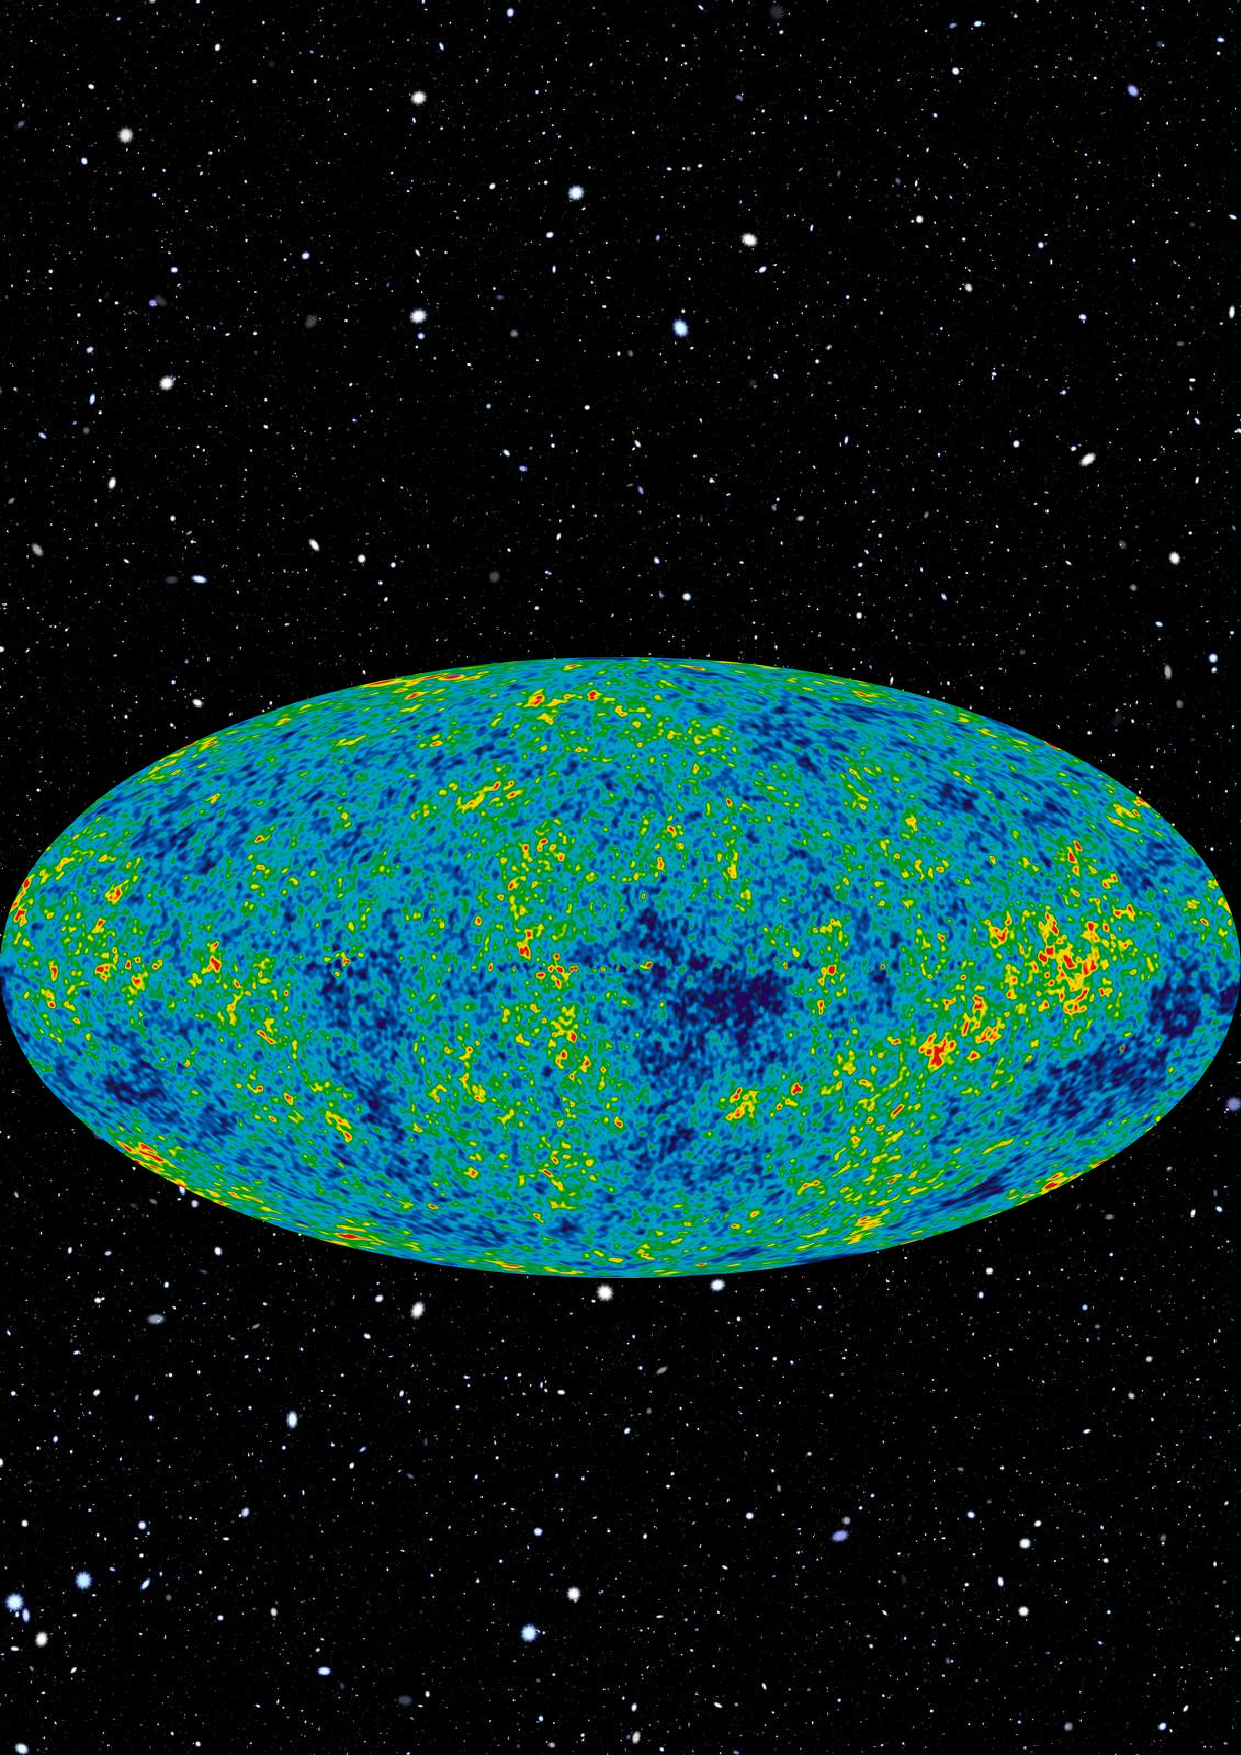
\includegraphics[width=\paperwidth,height=\paperheight,keepaspectratio]{Capa/Figuras_Capa/WMAP_Capa.pdf}
    };
\end{tikzpicture}

% Desenha um retângulo (branca)
\begin{tikzpicture}[remember picture, overlay]
    \draw[line width=7.4cm, white] 
        ($(current page.west) + (0,10.4)$) -- ($(current page.east) + (0,10.4)$);
\end{tikzpicture}

% Desenha um retângulo (cor da edição)
\begin{tikzpicture}[remember picture, overlay]
    \draw[line width=7cm, base] 
        ($(current page.west) + (0,10.4)$) -- ($(current page.east) + (0,10.4)$);
\end{tikzpicture}

% LOGO Lettering
% Altere a cor da logo de acordo com a cor usada para a Edição se for conveniente
\begin{tikzpicture}[remember picture, overlay]
  % Adiciona a imagem com um deslocamento usando shift
  \node at (current page.north west) [anchor=north west, xshift=2.85cm, yshift=-0.8cm] {
    
\includegraphics[width=15cm]{Capa/Figuras_Capa/Newston_Jornal_Logo_Lettering_Branca.png}
  };
\end{tikzpicture}

% Ajuste os valores em \textls[] (espaço entre letras) e na coordenada y de \node para adequar o tema e número com data da edição dentro do retângulo
\begin{tikzpicture}[remember picture, overlay]
    \node[anchor=north] at ($(current page.north west) + (0.5cm,-1.15cm)$) {
        \rotatebox{90}{\sffamily\bfseries\myfontsizeTemaCapaVerticalECC \textls[10]{HISTÓRIA\, DO\, UNIVERSO}}
    };
\end{tikzpicture}

\begin{tikzpicture}[remember picture, overlay]
    \node[anchor=north] at ($(current page.north west) + (20.5cm,-1.1cm)$) {
        \rotatebox{90}{{\sffamily\bfseries\myfontsizeTemaCapaVerticalECC \textls[10]{EDIÇÃO \NumeroEdicao -}} {\sffamily\myfontsizeTemaCapaVerticalECC\textls[10]{\MakeUppercase{\DataEdicao}}}}
    };
\end{tikzpicture}

% Tema da edição
\vspace{1.7cm}
\hspace{-1.5cm}{\sffamily\bfseries\myfontsizeTema\echoShadowText{baseechoshadow}{baseshadow}{História do Universo:}}

% Logo da UEM Branco
\begin{tikzpicture}[remember picture, overlay]
    % Ajuste a posição da figura conforme necessário
    \node[anchor=south, yshift=19.5cm, xshift=8.5cm] at (current page.south) { % Deslocamento vertical e horizontal na página - altere de acordo com o local em que deseja posicionar a logo
        
\includegraphics[width=0.17\textwidth]{Capa/Figuras_Capa/UEM_Logo_Modelo_Branco.png}
    };
\end{tikzpicture}

\begin{tikzpicture}[remember picture, overlay]
    \node[anchor=center, inner sep=0pt, outer sep=0pt] at ([shift={(-1.5cm,-8.5cm)}] current page.center) {
        \begin{tikzpicture}
             % Texto principal com contorno
            \node[anchor=center, inner sep=0pt, outer sep=0pt] {
                {\sffamily\bfseries\myfontsizeTituloTema \contour{base}{\shortstack[l]{ERA\\[0.5ex] PRIMORDIAL}}}
            };
        \end{tikzpicture}
    };
\end{tikzpicture}


% Desenha um retângulo (branca)
\begin{tikzpicture}[remember picture, overlay]
    \draw[line width=1.9cm, white] 
        ($(current page.west) + (0,-12.8)$) -- ($(current page.east) + (0,-12.8)$);
\end{tikzpicture}

% Desenha um retângulo (cor da edição) que engloba um título de artigo (diminua ou aumente a coordenada em x do segundo conjunto de coordenadas)
\begin{tikzpicture}[remember picture, overlay]
    \draw[line width=1.7cm, base] 
        ($(current page.west) + (0.1,-12.8)$) -- ($(current page.east) + (-12,-12.8)$);
\end{tikzpicture}

% Títulos de Artigos na Capa com TikZ (altere as coordenadas para posicionar o título do artigo dentro do retângulo de sua preferência)
\begin{tikzpicture}[remember picture, overlay]
    \node[anchor=north west, inner sep=0pt, outer sep=0pt] at ($(current page.north west) + (0.5cm,-27.2cm)$) {
        {\sffamily\bfseries\myfontsizeTitulosArtigosCapa À Luz de Caravaggio}
    };
\end{tikzpicture}


% Desenha um retângulo (cor da edição) que engloba um título de artigo (diminua ou aumente a coordenada em x do primeiro e segundo conjunto de coordenadas)
\begin{tikzpicture}[remember picture, overlay]
    \draw[line width=1.7cm, base] 
        ($(current page.west) + (9.1,-12.8)$) -- ($(current page.east) + (-6.5,-12.8)$);
\end{tikzpicture}

% Títulos de Artigos na Capa com TikZ (altere as coordenadas para posicionar o título do artigo dentro do retângulo de sua preferência) para textos em duas linhas use \myfontsizeTitulosArtigosCapaDois para diminuir o tamanho da fonte
\begin{tikzpicture}[remember picture, overlay]
    \node[anchor=north west, inner sep=0pt, outer sep=0pt, text width=10cm] at ($(current page.north west) + (10.1cm,-27cm)$) {
        {\sffamily\bfseries\myfontsizeTitulosArtigosCapaDois Tipos de \\ Radiações}
    };
\end{tikzpicture}

\begin{tikzpicture}[remember picture, overlay]
    \draw[line width=1.7cm, base] 
        ($(current page.west) + (14.6,-12.8)$) -- ($(current page.east) + (-0.1,-12.8)$);
\end{tikzpicture}

\begin{tikzpicture}[remember picture, overlay]
    \node[anchor=north west, inner sep=0pt, outer sep=0pt, text width=10cm] at ($(current page.north west) + (15.7cm,-27cm)$) {
        {\sffamily\bfseries\myfontsizeTitulosArtigosCapaDois A Física dos\\[0.5ex] Esportes}
    };
\end{tikzpicture}

    \newpage
\thispagestyle{empty}
% OBS: Coloque sempre o que você quer deixar de fundo na página como primeiro comando

% Imagem de fundo - crie um arquivo separado em tamanho A4 (210x297mm) no formato pdf
\begin{tikzpicture}[remember picture,overlay]
    % Inclui a imagem em segundo plano
    \node[anchor=center,inner sep=0pt] at (current page.center) {
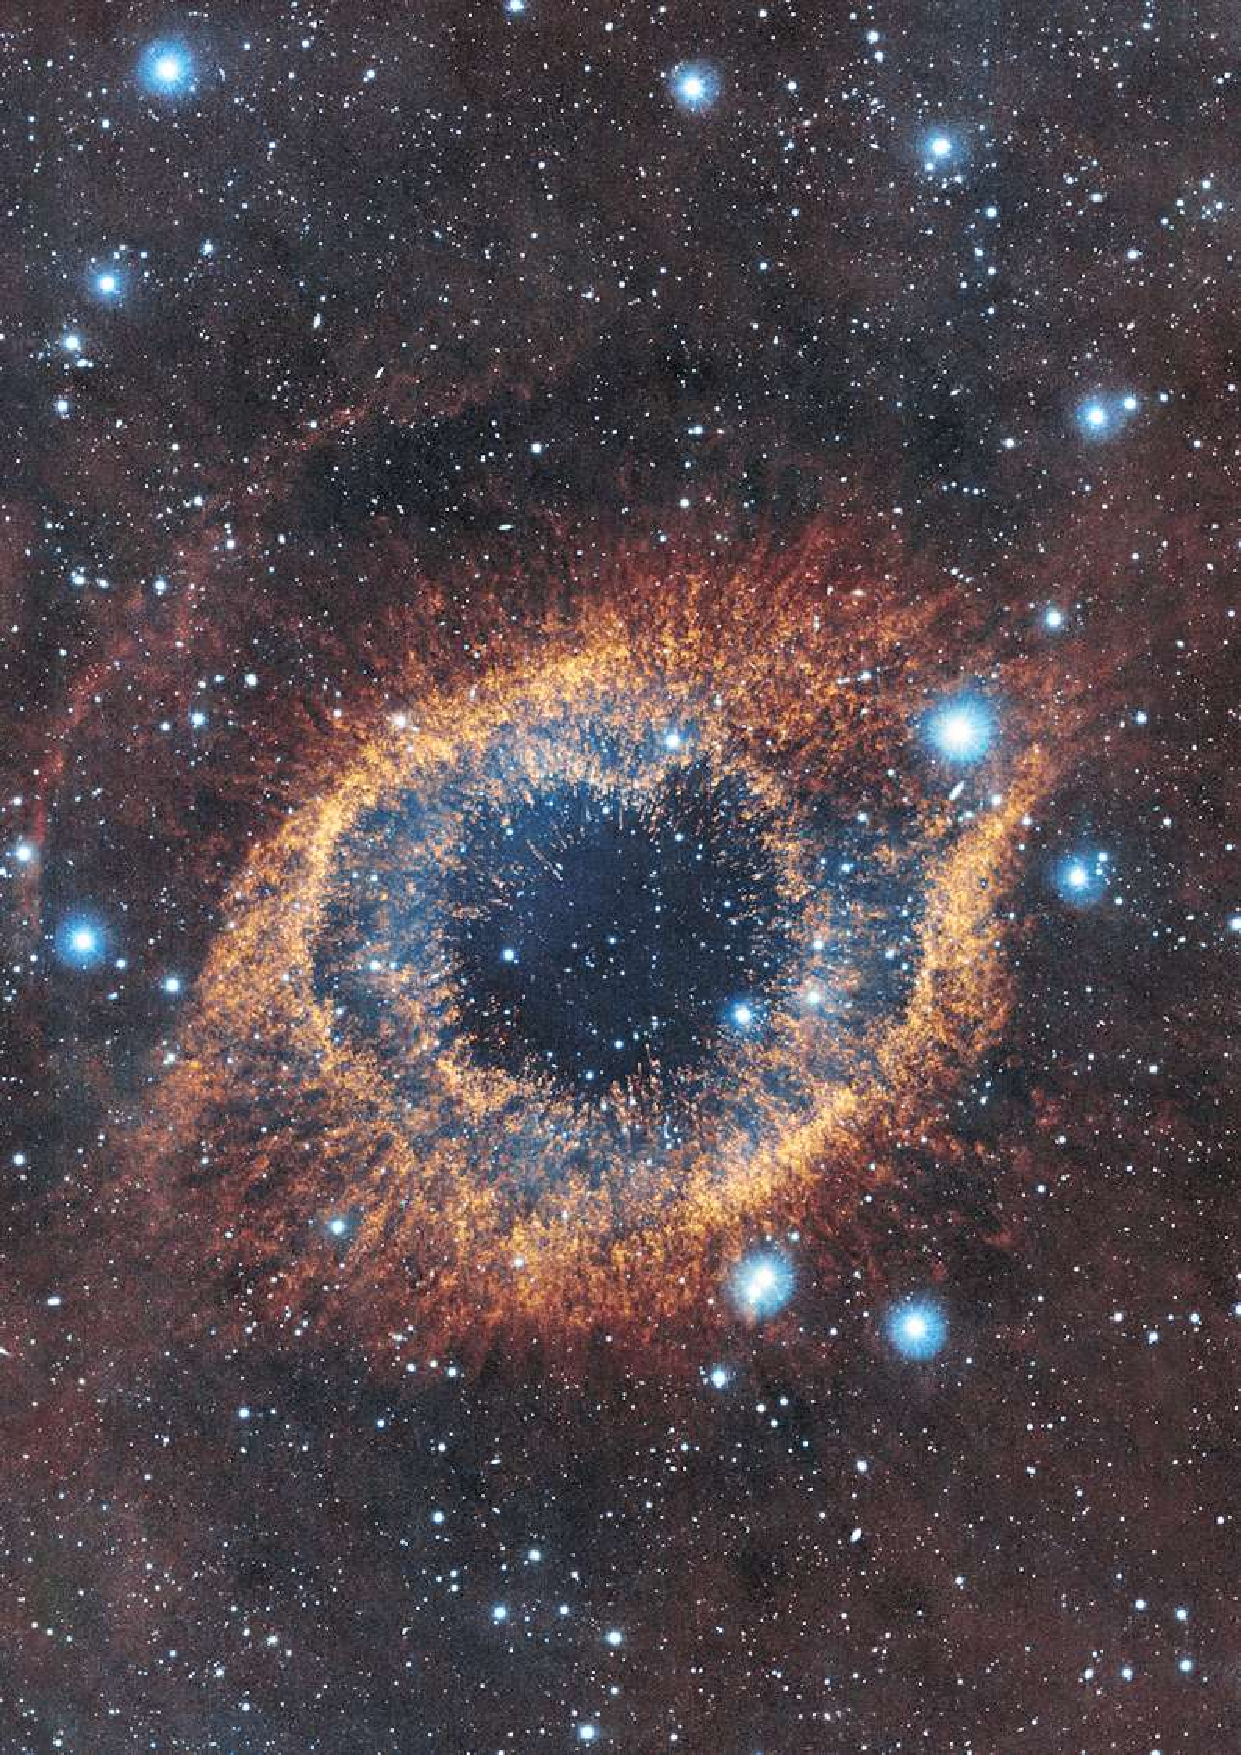
\includegraphics[width=\paperwidth,height=\paperheight,keepaspectratio]{Folha_Rosto/Figs_Folha_Rosto/HelixNebula.pdf}
    };
\end{tikzpicture}

% Marcador de página branco
\begin{tikzpicture}[remember picture, overlay, x=1.1pt, y=1.1pt, yscale=-1, xscale=1]
    % Desenho do triângulo com altura aumentada
    \begin{scope}[yshift=-3cm, xshift=-7cm]
        \draw[fill=white, draw=white] 
            (181.51,363.13) -- (181.51,-192.01) -- (390.86,-192.01) -- 
            (390.86,363.13) -- (285.98,431.63) -- (181.56,363.13) -- 
            (181.51,363.13) -- cycle;
    \end{scope}
\end{tikzpicture}

%LOGO 
% Altere a cor da logo de acordo com a cor usada para a Edição se for conveniente
\begin{tikzpicture}[remember picture, overlay]
  % Adiciona a imagem com um deslocamento usando shift
  \node at (current page.north west) [anchor=north west, xshift=3cm, yshift=-0.9cm] {
    
\includegraphics[width=7.2cm]{Folha_Rosto/Figs_Folha_Rosto/Logo_Na_Cor_Da_Edicao.png}
  };
\end{tikzpicture}

%Número da Edição, coleção (se houver) e data (mês ano)
\begin{tikzpicture}[remember picture, overlay]
  % Desenhar a primeira linha
  \draw[line width=1mm, color=base, shift={(2, -2.3)}] (-1.3,-1) -- (5.4,-1);

  % Adicionar o círculo no meio da linha com um número dentro e preenchido com a cor base
  \node[circle, draw=base, fill=base, minimum size=1cm, inner sep=0pt, text=white, shift={(2, -2.3)}] at (2,-1) {\sffamily\bfseries\myfontsizeEditionFolhaRosto \NumeroEdicao};

  % Adicionar a palavra "Coleção" entre as duas linhas
  \node[shift={(2, -2.8)}, anchor=center] at (0,-1) {\sffamily\bfseries \myfontsizeColecaoData COLEÇÃO \ColecaoEdicao};

  % Adicionar outra palavra ao lado de "Coleção"
  \node[shift={(2, -2.8)}, anchor=center] at (4,-1) {\sffamily\bfseries \myfontsizeColecaoData \MakeUppercase{\DataEdicao}};

  % Desenhar a segunda linha
  \draw[line width=1mm, color=base, shift={(2, -3.3)}] (-1.3,-1) -- (5.4,-1);

   % Desenhar uma linha pontilhada
   \foreach \i in {0.8, 0.95, 1.10, 1.25, 1.40, 1.55, 1.70, 1.85, 2, 2.15, 2.30, 2.45, 2.60, 2.75, 2.90, 3.05, 3.20} {
  \fill[base, shift={(0, -4)}] (\i+2, -1) circle (1pt);
};
  % Tema Principal
  \node[shift={(0, -5.8)}, anchor=center] at (4, -1) {
    \parbox{7cm}{\centering \sffamily\bfseries \myfontsizeColecaoTema HISTÓRIA DO\\[1.5ex]UNIVERSO:\\[1.5ex]ERA PRIMORDIAL}
  }; % Aumente o parâmetro em \parbox para caber mais texto, se for necessário
  
  % Desenhar uma linha pontilhada
   \foreach \i in {0.8, 0.95, 1.10, 1.25, 1.40, 1.55, 1.70, 1.85, 2, 2.15, 2.30, 2.45, 2.60, 2.75, 2.90, 3.05, 3.20} {
  \fill[base, shift={(0, -7.7)}] (\i+2, -1) circle (1pt);
};
  % Logo UEM
   \node[shift={(0, -9)}, anchor=center] at (4, -1) {
\includegraphics[width=0.15\textwidth]{Folha_Rosto/Figs_Folha_Rosto/UEM_Logo_Modelo_Colorido.png}
    };
\end{tikzpicture}


% Tipo do jornal
\begin{tikzpicture}[remember picture, overlay]
  % Tema Principal
  \node[shift={(4.1, -15.8)}, anchor=center] at (5.7, -1) {
    \parbox{20cm}{\sffamily\bfseries\myfontsizeDivulgacaoCientifica\textls[150]{DIVULGAÇÃO\\[0.4ex]CIENTÍFICA\\[1ex]E CULTURAL\\[1ex] PARA A\\[1ex]COMUNIDADE}}
  };
\end{tikzpicture}


    \newpage
\thispagestyle{noheader}
% OBS: Coloque sempre o que você quer deixar de fundo na página como primeiro comando
% Adicione o TikZ para desenhar a linha vertical
\begin{tikzpicture}[remember picture, overlay]
    \draw[line width=10.8cm, base] ($(current page.north east) - (0,0)$) -- ($(current page.south east) - (0,0)$);
\end{tikzpicture}

\begin{tikzpicture}[remember picture, overlay]
  \node[shift={(-0.2, 2.2)}, anchor=center] at (4,-1) {\usefont{T1}{qag}{b}{n} {\myfontsizeSdeSumario S}\myfontsizeSumario umário};
  \node[shift={(-2.6, 0.2)}, anchor=center] at (4,-1) {\sffamily\bfseries\myfontsizeSumarioData \DataEdicao};
\end{tikzpicture}

% Adiciona um espaço vertical negativo para mover o sumário para cima
\vspace*{-0.2cm} % Ajuste este valor conforme necessário para que caibam mais itens de sumário numa mesma página

% Ajustar a largura do sumário usando adjustbox
\makebox[0pt][l]{
    \begin{adjustbox}{valign=t,minipage={.8\textwidth},margin={-3.5em,0pt}}
        {\myfontsizeSumarioTitulos\sffamily
       \tableofcontents}
    \end{adjustbox}
}

%LOGO, NOME DO JORNAL e outras informações do canto direito da página de Sumário
%Edite a imagem em um editor gráfico antes de incluí-la no documento LaTeX. Ferramentas como GIMP, Inkscape, ou Photoshop podem ser usadas para alterar a cor da imagem (use o arquivo svg da pasta Figs_Folha_Rosto).
% Altere a cor e/ou tamanho no comando \myfontsizeNewstonSumario \myfontsizeJornalSumarioECC em Structure.tex caso queira outra que não seja a da edição
\begin{tikzpicture}[remember picture, overlay]
  % Adiciona a logo maçã branco
  \node at (current page.north west) [anchor=north west, xshift=15.4cm, yshift=-0.7cm] {
    
\includegraphics[width=5.5cm]{Sumario/Figs_Sumario/Newston_Logo_Branca.png}
  };
   % Adiciona o texto Edições Anteriores
  \node at (current page.north west) [anchor=north west, xshift=16.25cm, yshift=-7.5cm] {
    \parbox{20cm}{\sffamily\bfseries\myfontsizeEdAntSite ACESSE AS EDIÇÕES \\[0.4ex] ANTERIORES}
  };
   % Ícone site
   \node at (current page.north west) [anchor=north west, xshift=16.25cm, yshift=-8.6cm] {
    
\includegraphics[width=.5cm]{Sumario/Figs_Sumario/Icone_Site.png}
  };
  % Site
  \node at (current page.north west) [anchor=north west, xshift=16.9cm, yshift=-8.75cm] {
    {\sffamily\myfontsizeEdAntSite www.newston.com.br}
  };
  % Ícone google drive
  \node at (current page.north west) [anchor=north west, xshift=16.2cm, yshift=-9.3cm] {
    
\includegraphics[width=.6cm]{Sumario/Figs_Sumario/Icone_GDrive.png}
  };
  % Pasta drive compartilhada
  \node at (current page.north west) [anchor=north west, xshift=16.8cm, yshift=-9.5cm] {
    {\sffamily\myfontsizeEdAntSite\textls[0]{\begingroup
\hypersetup{urlcolor=white}  % Altera a cor do link apenas para este caso
\href{https://drive.google.com/drive/folders/1FbL4MqIMpF6chux5QbDVhHFrDrhzHxMa?usp=drive_link}{Drive Newston}
\endgroup}}
  };
  % Adiciona o texto Fale Conosco...
  \node at (current page.north west) [anchor=north west, xshift=16.25cm, yshift=-20.3cm] {
    \parbox{20cm}{\sffamily\bfseries\myfontsizeEdAntSite FALE CONOSCO POR \\[0.8ex] NOSSAS REDES \\[0.8ex] SOCIAIS}
  };
  % Ícone Insta
   \node at (current page.north west) [anchor=north west, xshift=16.25cm, yshift=-21.8cm] {\href{https://www.instagram.com/newstonjornal/}{
\includegraphics[width=.6cm]{Sumario/Figs_Sumario/Icone_Insta.png}}
  };
  % Ícone Face
   \node at (current page.north west) [anchor=north west, xshift=17.25cm, yshift=-21.8cm] {\href{https://www.facebook.com/newstonjornal}{
\includegraphics[width=.6cm]{Sumario/Figs_Sumario/Icone_Facebook.png}}
  };
  % Ícone X
   \node at (current page.north west) [anchor=north west, xshift=18.25cm, yshift=-21.8cm] {\href{https://x.com/newstonjornal}{
\includegraphics[width=.6cm]{Sumario/Figs_Sumario/Icone_X.png}}
  };
  % Usuario
  \node at (current page.north west) [anchor=north west, xshift=16.25cm, yshift=-22.7cm] {
    {\sffamily\myfontsizeUsuario \textls[100]{@NEWSTONJORNAL}}
  };
  % Ícone e-mail
   \node at (current page.north west) [anchor=north west, xshift=16.25cm, yshift=-23.3cm] {
    
\includegraphics[width=.5cm]{Sumario/Figs_Sumario/Icone_Email.png}
  };
  % e-mail
  \node at (current page.north west) [anchor=north west, xshift=16.8cm, yshift=-23.38cm] {
    {\sffamily\myfontsizeEdAntSite \textls[0]{\begingroup
\hypersetup{urlcolor=white}  % Altera a cor do link apenas para este caso
\href{mailto:newstonjornal@gmail.com}{newstonjornal@gmail.com}
\endgroup}}
  };
  % Adiciona a logo da UEM branco
  \node at (current page.north west) [anchor=north west, xshift=16.2cm, yshift=-26.7cm] {
    
\includegraphics[width=3.7cm]{Capa/Figuras_Capa/UEM_Logo_Modelo_Branco.png}
  };
\end{tikzpicture}
    \newpage
\thispagestyle{noheader}
% Adicione o TikZ para desenhar a linha vertical
\begin{tikzpicture}[remember picture, overlay]
    \draw[line width=3.4cm, base] ($(current page.north east) - (0,0)$) -- ($(current page.south east) - (0,0)$);
\end{tikzpicture}

\noindent{\sffamily\myfontsizeequipe\textls[100]{\textbf{EQUIPE}}}

\vspace{0.3cm} 
\noindent{\hspace{0.05cm}\sffamily\myfontsizecolabbebas
\textls[100]{COLABORADORES\, DO\, JORNAL}
}

\vspace{0.3cm} 
% Número da Edição
    \noindent{\hspace{0.05cm}\sffamily\myfontsizeEdition
    \textls[100]{\textbf{Newston Jornal - Ed. \NumeroEdicao}}
    }
    
\vspace{0.3cm} 
% Mês e ano da Edição
\noindent{\hspace{0.05cm}\sffamily\myfontsizeEdition
    \textls[100]{\DataEdicao}}

\vspace{1cm}
% Para adicionar novo colaborador copie e cole o ambiente a seguir logo abaixo e faça as devidas alterações. Na parte do e-mail mantenha "mailto:" antes do e-mail para que ao clicar sobre o e-mail no PDF o leitor seja direcionado para sua caixa de e-mail padrão.

% Colaborador 01
\begin{itemize}
    \item {\sffamily\myfontsizeColaboradores \textls[100]{\textbf{Nome Completo do Colaborador 1}}} % Nome
    {\sffamily\myfontsizeColaboradores \textls[100]{(\href{mailto:emailcol1@email.com}{emailcol1@email.com})}} % E-mail
    \begin{itemize}[label={\raisebox{0.4ex}{\color{black}\scalebox{0.3}{\textcircled{\color{white}\textbullet}}}}, labelsep=0.5em] % Define o símbolo como um círculo branco com contorno preto
        \item {\sffamily\myfontsizeColaboradores \textls[100]{Cargo no jornal (Ex: Editor, revisor) - Título ou cargo, departamento e sigla da Universidade --- exemplos a seguir.}}% Cargo na revista - Formação acadêmica e/ou Departamento/Universidade 
    \end{itemize}
\end{itemize}

% Colaborador 02
\begin{itemize}
    \item {\sffamily\myfontsizeColaboradores \textls[100]{\textbf{Mickey Mouse}}} % Nome
    {\sffamily\myfontsizeColaboradores \textls[100]{(\href{mailto:mickeymouse@email.com}{mickeymouse@email.com})}} % E-mail
    \begin{itemize}[label={\raisebox{0.4ex}{\color{black}\scalebox{0.3}{\textcircled{\color{white}\textbullet}}}}, labelsep=0.5em] % Define o símbolo como um círculo branco com contorno preto
        \item {\sffamily\myfontsizeColaboradores \textls[100]{Orientador - Professor DFI/UEM}}% Cargo na revista - Formação acadêmica e/ou Departamento/Universidade 
    \end{itemize}
\end{itemize}

% Colaborador 03
\begin{itemize}
    \item {\sffamily\myfontsizeColaboradores \textls[100]{\textbf{Tintim}}} % Nome
    {\sffamily\myfontsizeColaboradores \textls[100]{(\href{mailto:tintim@email.com}{tintim@email.com})}} % E-mail
    \begin{itemize}[label={\raisebox{0.4ex}{\color{black}\scalebox{0.3}{\textcircled{\color{white}\textbullet}}}}, labelsep=0.5em] % Define o símbolo como um círculo branco com contorno preto
        \item {\sffamily\myfontsizeColaboradores \textls[100]{Editor - Doutorando em Física/UEL}}% Cargo na revista - Formação acadêmica e/ou Departamento/Universidade 
    \end{itemize}
\end{itemize}

% Colaborador 04
\begin{itemize}
    \item {\sffamily\myfontsizeColaboradores \textls[100]{\textbf{Marinheiro Popeye}}} % Nome
    {\sffamily\myfontsizeColaboradores \textls[100]{(\href{mailto:popeye@email.com}{popeye@email.com})}} % E-mail
    \begin{itemize}[label={\raisebox{0.4ex}{\color{black}\scalebox{0.3}{\textcircled{\color{white}\textbullet}}}}, labelsep=0.5em] % Define o símbolo como um círculo branco com contorno preto
        \item {\sffamily\myfontsizeColaboradores \textls[100]{Revisor - Arquitetura e Urbanismo/UEM}}% Cargo na revista - Formação acadêmica e/ou Departamento/Universidade 
    \end{itemize}
\end{itemize}







    % PRIMEIRO ARTIGO
\newcommand{\titleone}{Título Principal - Artigo 1} % Título do Artigo (basta colocar o título nessa linha que automaticamente irá aparecer no cabeçalho e sumário, referentes ao artigo, e também nas referências). Altere o nome \titleone para \titletwo, \titlethree e assim por diante de acordo com o total de artigos da edição. Faça o mesmo sempre que aparecer \titleone nos comandos abaixo e em outros arquivos tex (como o de referências). 
\mytitle{\titleone}    
\addchaptersummary{\titleone}{Sumario/Figs_Sumario/FigArtigo1.jpg}{O Vapor Willie é um curta-metragem em preto e branco da Walt Disney Studios de 1928 estrelado por Mickey Mouse e dirigido por Walt Disney e Ub Iwerks.}{Mickey Mouse} 
% Comando para adicionar o título do artigo (deve ficar após o comando \mytitle) no sumário bem como uma figura, resumo e autor(a) do mesmo, respectivamente (obs: o diretório da figura deve ser especificado na segunda variável como mostra esse exemplo com "Sumario/Figs_Sumario/FigArtigo1.jpg". Recomenda-se o uso de figuras quadradas para adicionar ao sumário.)
\newcommand{\refarticleone}{\titleone} % Comando para adicionar o nome do artigo nas referências. Altere \refarticleone para \refarticletwo, \refarticlethree de acordo com o total de artigos da edição e adicione o mesmo comando antes da sua respectiva seção no arquivo Referencias.tex


% Use o ambiente multicols para textos em duas colunas.
\begin{multicols}{2} % Tudo o que estiver dentro desse ambiente ficará no layout de duas colunas. 
% Pule uma linha entre \begin{multicols} e o texto

O título principal do Artigo em questão quando incluído no comando referente ao título aparecerá automaticamente no cabeçalho, no sumário e também no título das referências.

Troque a cor do layout em \texttt{\textbackslash definecolor\{base\}\{HTML\}\{HEX da cor\}\}} na parte referente as cores do arquivo Structure.tex. Outras informações e comandos podem ser visualizados no arquivo Tex em mais detalhes. A seguir mencionamos alguns comandos básicos também no arquivo PDF. 

Para um novo subtítulo use: \texttt{\textbackslash mysubtitle\{Subtítulo 1: Artigo 1\}}. 
%
\mysubtitle{Subtítulo 1: Artigo 1} % Subtítulo do Artigo  
%

Para citar links externos use o comando \texttt{\textbackslash href\{linkhttps\}\{Palavra clicável no texto\}}. Um exemplo na prática pode ser visualizado na legenda para a primeira figura a seguir. Use o ambiente \texttt{figure} para adicionar figuras ao artigo. 

\begin{figure}[H]
	\centering
	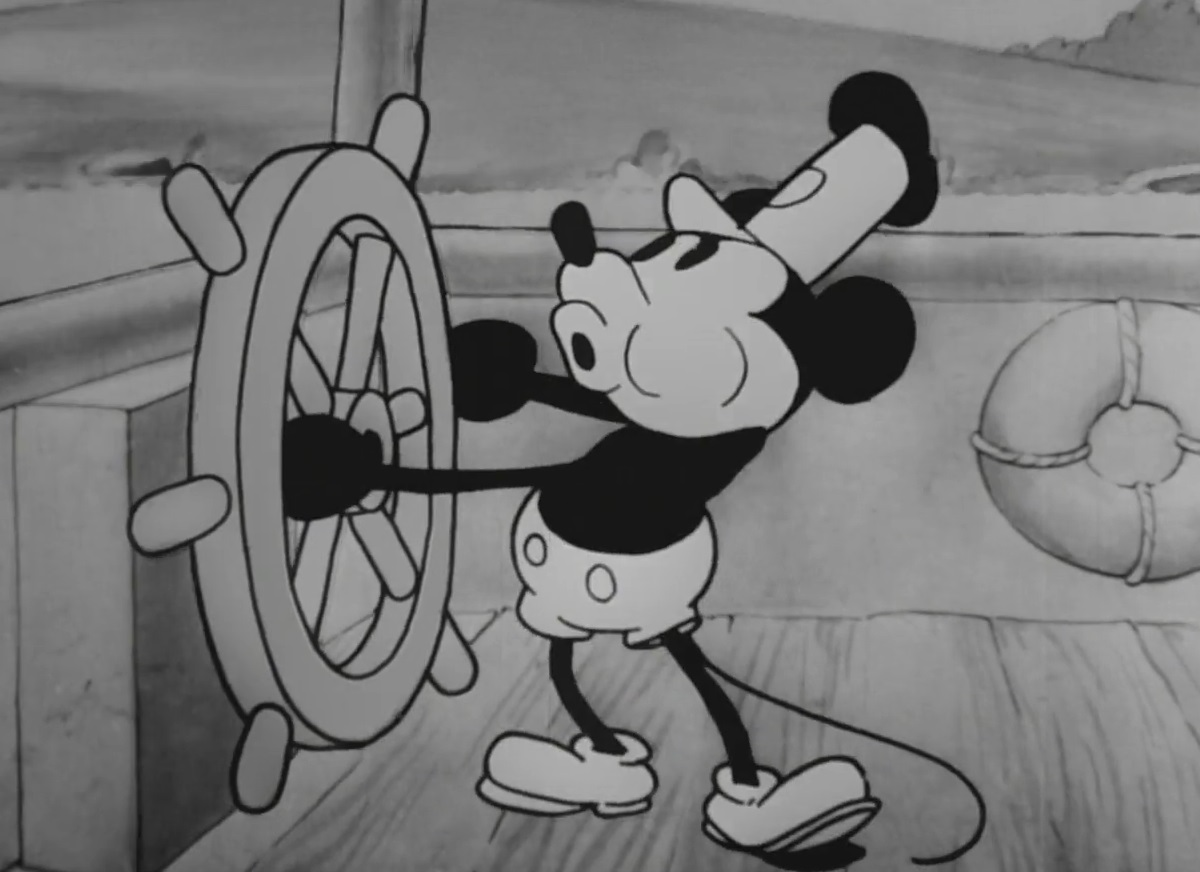
\includegraphics[width=\linewidth]{Figuras/Artigo1/Mickey.jpg}
	\caption{Mickey Mouse pilotando o Vapor Willie. Fonte: \href{https://www.cnnbrasil.com.br/entretenimento/o-mickey-vai-entrar-em-dominio-publico-em-2024-o-que-vai-mudar/}{CNN Brasil}.}
	\label{fig:mickeymouse}
\end{figure}

Cite figuras usando o comando \texttt{\textbackslash ref\{fig:mickeymouse\}}, sendo o rótulo da Figura definido no ambiente \textit{figure} por \texttt{\textbackslash label\{fig:mickeymouse\}}. Na prática: Aqui eu cito a Figura \ref{fig:mickeymouse}.

Para aspas duplas de abertura, use dois caracteres de acento grave (ou crase) e para aspas duplas de fechamento, use dois caracteres de aspas simples. Ex: ``palavra ou frase''. Use o comando \texttt{\textbackslash footnote\{\}} para notas de rodapé (Ex: Veja essa nota\footnote{Aqui temos uma nota de rodapé.}).

Para equações use o ambiente \textit{equation}:
%
\begin{equation}\label{Eq1}
    E = \frac{hc}{\lambda},
\end{equation}
%
em que $h$ é a constante de Planck e $c$ a velocidade da luz no vácuo.

Use o comando \texttt{\textbackslash noindent} para tirar a indentação de um parágrafo ou o símbolo de porcentagem entre o \texttt{\textbackslash end\{equation\}} e a próxima linha de texto. Para citar equações numeradas no texto você também pode fazer uso do comando \texttt{\textbackslash ref\{Eq1\}} para citar a equação no texto de acordo com o seu rótulo no comando \texttt{\textbackslash label\{Eq1\}}. Aqui eu cito a Equação \ref{Eq1}.




\mysubtitle{Subtítulo 2: Artigo 1}

\lipsum[1]

Para citar uma referência apenas use o comando:

\texttt{\textbackslash ref\{ref1\}}. 

\noindent Onde em \texttt{ref1} coloco a etiqueta que conecta à referência 1 do artigo 1 definida no documento \texttt{Referencias.tex.}

\noindent\textbf{Exemplo:} aqui eu cito \textbf{uma referência} do artigo 1 \ref{ref1:artigo1}.

Para citar duas referências use o comando:

\noindent\texttt{\textbackslash refdois\{ref2\}\{ref3\}}

\noindent \textbf{Exemplo:} aqui eu cito \textbf{duas referências} para o artigo 1 \refdois{ref2:artigo1}{ref3:artigo1}.

Para citar três referências use o comando:

\noindent\texttt{\textbackslash reftres\{ref2\}\{ref3\}\{ref4\}}

\noindent \textbf{Exemplo}: aqui eu cito \textbf{três referências} para o artigo 1 \reftres{ref2:artigo1}{ref3:artigo1}{ref4:artigo1}.

Para 4 ou mais referências em um mesmo parágrafo você deve criar um comando específico, seguindo a lógica dos comandos já criados, de acordo com as suas especificações no arquivo \texttt{Structure.tex}. Observe que mesmo se as referências não forem citadas no texto, elas ainda aparecem na Seção Referências do PDF, como ocorre para as referências dos Artigos 2 e 3 usadas como exemplo.








Use o comando \texttt{\textbackslash authorinfo\{Nome do autor do artigo\}\{link https do seu lattes ou do seu ORCID\}} no final do artigo em questão para referenciar o autor.

\authorinfo{Mickey Mouse}{link lattes ou orcid}
% Use esse comando para adicionar o nome do autor(a) do artigo no final, e o link para o seu currículo lattes ou orcid




\end{multicols}

 % Use essa linha de comando para adicionar novos artigos (recomenda-se criar um arquivo .tex para cada artigo)
    % SEGUNDO ARTIGO
\newcommand{\titletwo}{Título Principal - Artigo 2} 
\mytitle{\titletwo}    
\addchaptersummary{\titletwo}{Sumario/Figs_Sumario/FigArtigo2.jpg}{Tintim é o protagonista de As Aventuras de Tintim, criada pelo quadrinista belga Hergé que estreou em 10 de janeiro de 1929.}{Tintim} 

\newcommand{\refarticletwo}{\titletwo} 

\begin{multicols}{2}

Para adicionar uma figura no \textit{layout} da página inteira, ou seja em uma coluna, basta fechar o ambiente \texttt{multicols} temporariamente. Use o comando \texttt{\textbackslash par \textbackslash noindent} para garantir que a imagem fique corretamente alinhada e evitar espaçamentos indesejados quando saímos do ambiente \texttt{multicols} e em seguida insira a figura com o ambiente \texttt{figure}. Exemplo a seguir.

\end{multicols}

\par\noindent
\begin{figure}[H]
    \centering
    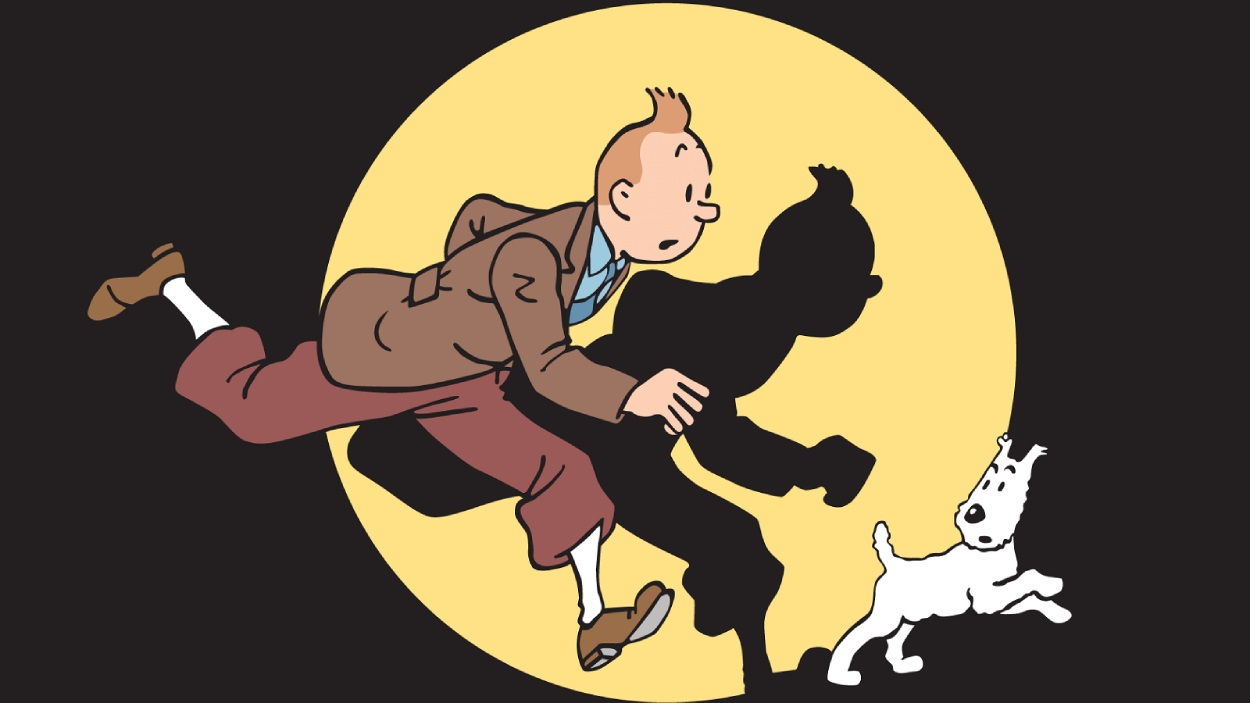
\includegraphics[width=\linewidth]{Figuras/Artigo2/Tintim.jpg}
    \caption{Tintim e seu inseparável amigo de 4 patas Bilu. Fonte: \href{https://br.pinterest.com/}{Pinterest}.}
    \label{fig:tintim}
\end{figure}


\begin{multicols}{2}
Para voltar ao \textit{layout} de duas colunas reinicie o ambiente \texttt{\textbackslash begin\{multicols\}\{2\}}. 

\lipsum[1-3]

\authorinfo{Tintim}{link lattes ou orcid}

\end{multicols}
    % TERCEIRO ARTIGO
\newcommand{\titlethree}{Título Principal - Artigo 3} 
\mytitle{\titlethree}    
\addchaptersummary{\titlethree}{Sumario/Figs_Sumario/FigArtigo3.jpg}{Popeye é um personagem de histórias em quadrinhos, criado por Elzie Crisler Segar. Sua primeira aparição foi em 17 de janeiro de 1929.}{Marinheiro Popeye} 

\newcommand{\refarticlethree}{\titlethree} 

\begin{multicols}{2}

\lipsum[1]

\begin{figure}[H]
	\centering
	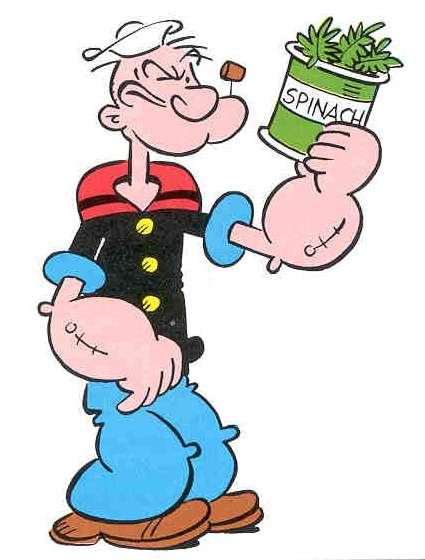
\includegraphics[width=\linewidth]{Figuras/Artigo3/Popeye.jpg}
	\caption{Popeye e sua fonte de força, o espinafre. Fonte: \href{https://br.pinterest.com/}{Pinterest}.}
	\label{fig:popeye}
\end{figure}

\mysubtitle{Subtítulo 1: Artigo 3}

\lipsum[1]

\authorinfo{Marinheiro Popeye}{link lattes ou orcid}

\end{multicols}
    % Título e referências na mesma página
\mytitle{Referências}% Título da seção de referências[]
\vspace{.5cm}
% Use \ref{ref1:artigo1} para citar uma referência no texto ou \refdois{ref1:artigo1}{ref2:artigo1} e \reftres{ref1:artigo1}{ref2:artigo1}{ref3:artigo1} para citar duas ou três referências.. para mais de três crie um ambiente parecido com o que define esses novos comandos em Structure.tex
\begin{center}
    \textcolor{base}{\MakeUppercase{\refarticleone}} % Não se esqueça de alterar \refarticleone para \refarticletwo e assim por diante para referências de outros artigos da edição
\end{center}

% Ambiente de referências, adicione uma referência para cada item. Não se esqueça de alterar a entrada em \label toda vez que for adicionar uma nova referência
\begin{enumerate}
    \item \label{ref1:artigo1} GUTH, Alan H. \textit{The Inflationary Universe: The Quest For a New Theory of Cosmic Origins}. [S.l.]: Helix Books, 1997. v. 33-57, Chapter 3: The birth of modern cosmology, p. 3357.
    \item \label{ref2:artigo1} RYDEN, Barbara. \textit{Introduction to cosmology}. [S.l.]: Cambridge University Press, 2017. 5.
    \item \label{ref3:artigo1} WEINBERG, Steven. \textit{Cosmology.} Oxford: Oxford University Press, 2008.
    \item \label{ref4:artigo1} DODELSON, Scott. \textit{Modern Cosmology.} Academic Press, 2003.
\end{enumerate}

% Referências Artigo 2
\begin{center}
    \textcolor{base}{\MakeUppercase{\refarticletwo}}
\end{center}

\begin{enumerate}
    \item \label{ref1:artigo2} BARLOW, R. J. Statistics: A Guide to the Use of Statistical Methods in the Physical Sciences. Wiley, 1989.
    \item \label{ref3:artigo2} GRIFFITHS, David J. \textit{Introduction to Electrodynamics.} 4. ed. Cambridge: Cambridge University Press, 2017.
\end{enumerate}

% Referências Artigo 3
\begin{center}
    \textcolor{base}{\MakeUppercase{\refarticlethree}}
\end{center}

\begin{enumerate}
    \item \label{ref1:artigo3} SAKURAI, J. J.; NAPOLITANO, Jim. Modern Quantum Mechanics. 2. ed. Cambridge: Cambridge University Press, 2017.
\end{enumerate}

% Referências para as figuras da capa e sumário

\begin{center}
    \textcolor{base}{\MakeUppercase{Figuras da Capa e Sumário}}
\end{center}

Figuras da capa: \href{https://www.britannica.com/science/cosmic-microwave-background}{CMB} e \href{https://www.canva.com/}{Fundo da capa};

Figura da contra-capa: \href{https://www.eso.org/public/images/eso1205a/}{Nebulosa Helix - EOS};

Figuras do sumário:

\begin{itemize}
    \item[i)] \href{https://pt.wikipedia.org/wiki/Steamboat_Willie}{\titleone};
    \item[ii)] \href{https://br.pinterest.com/}{\titletwo};
    \item[iii)] \href{https://br.pinterest.com/}{\titlethree};
\end{itemize}





    \newpage
\thispagestyle{empty}
% Adicione o TikZ para desenhar a linha vertical
\begin{tikzpicture}[remember picture, overlay]
    \draw[line width=3.4cm, base] ($(current page.north east) - (0,0)$) -- ($(current page.south east) - (0,0)$);
\end{tikzpicture}

\vspace{-1cm} % Espaço vertical para mover a figura para cima e caber na página (ajuste de acordo com o modelo, mantendo na página com uma linha vertical de cor referente a base)
\noindent % Evita indentação
\begin{minipage}{7.7cm}% Define a largura da minipage igual à largura da figura
\protect\vspace{16.5cm}% Ajuste fino para mover nota verticalmente
  \large{{\bfseries\sffamily Nota do autor:} \sffamily Os outros personagens que aparecem nesta tirinha são o Prof. Cloro e Estrôncio, que também estão em outras tirinhas de minha criação. Aqui, apresenta-se a origem do Sir Apple em uma coletânea de tirinhas especiais. A história continua...}
\end{minipage}
\hspace*{\fill} % Empurra a figura para a direita (caso não use a nota do autor então evite pular linha entre o \end{tikzpicture} da linha vertical e \hspace*{\fill} )
% Tirinha 
\begin{minipage}{9cm} % Define a largura da minipage igual à largura da figura
    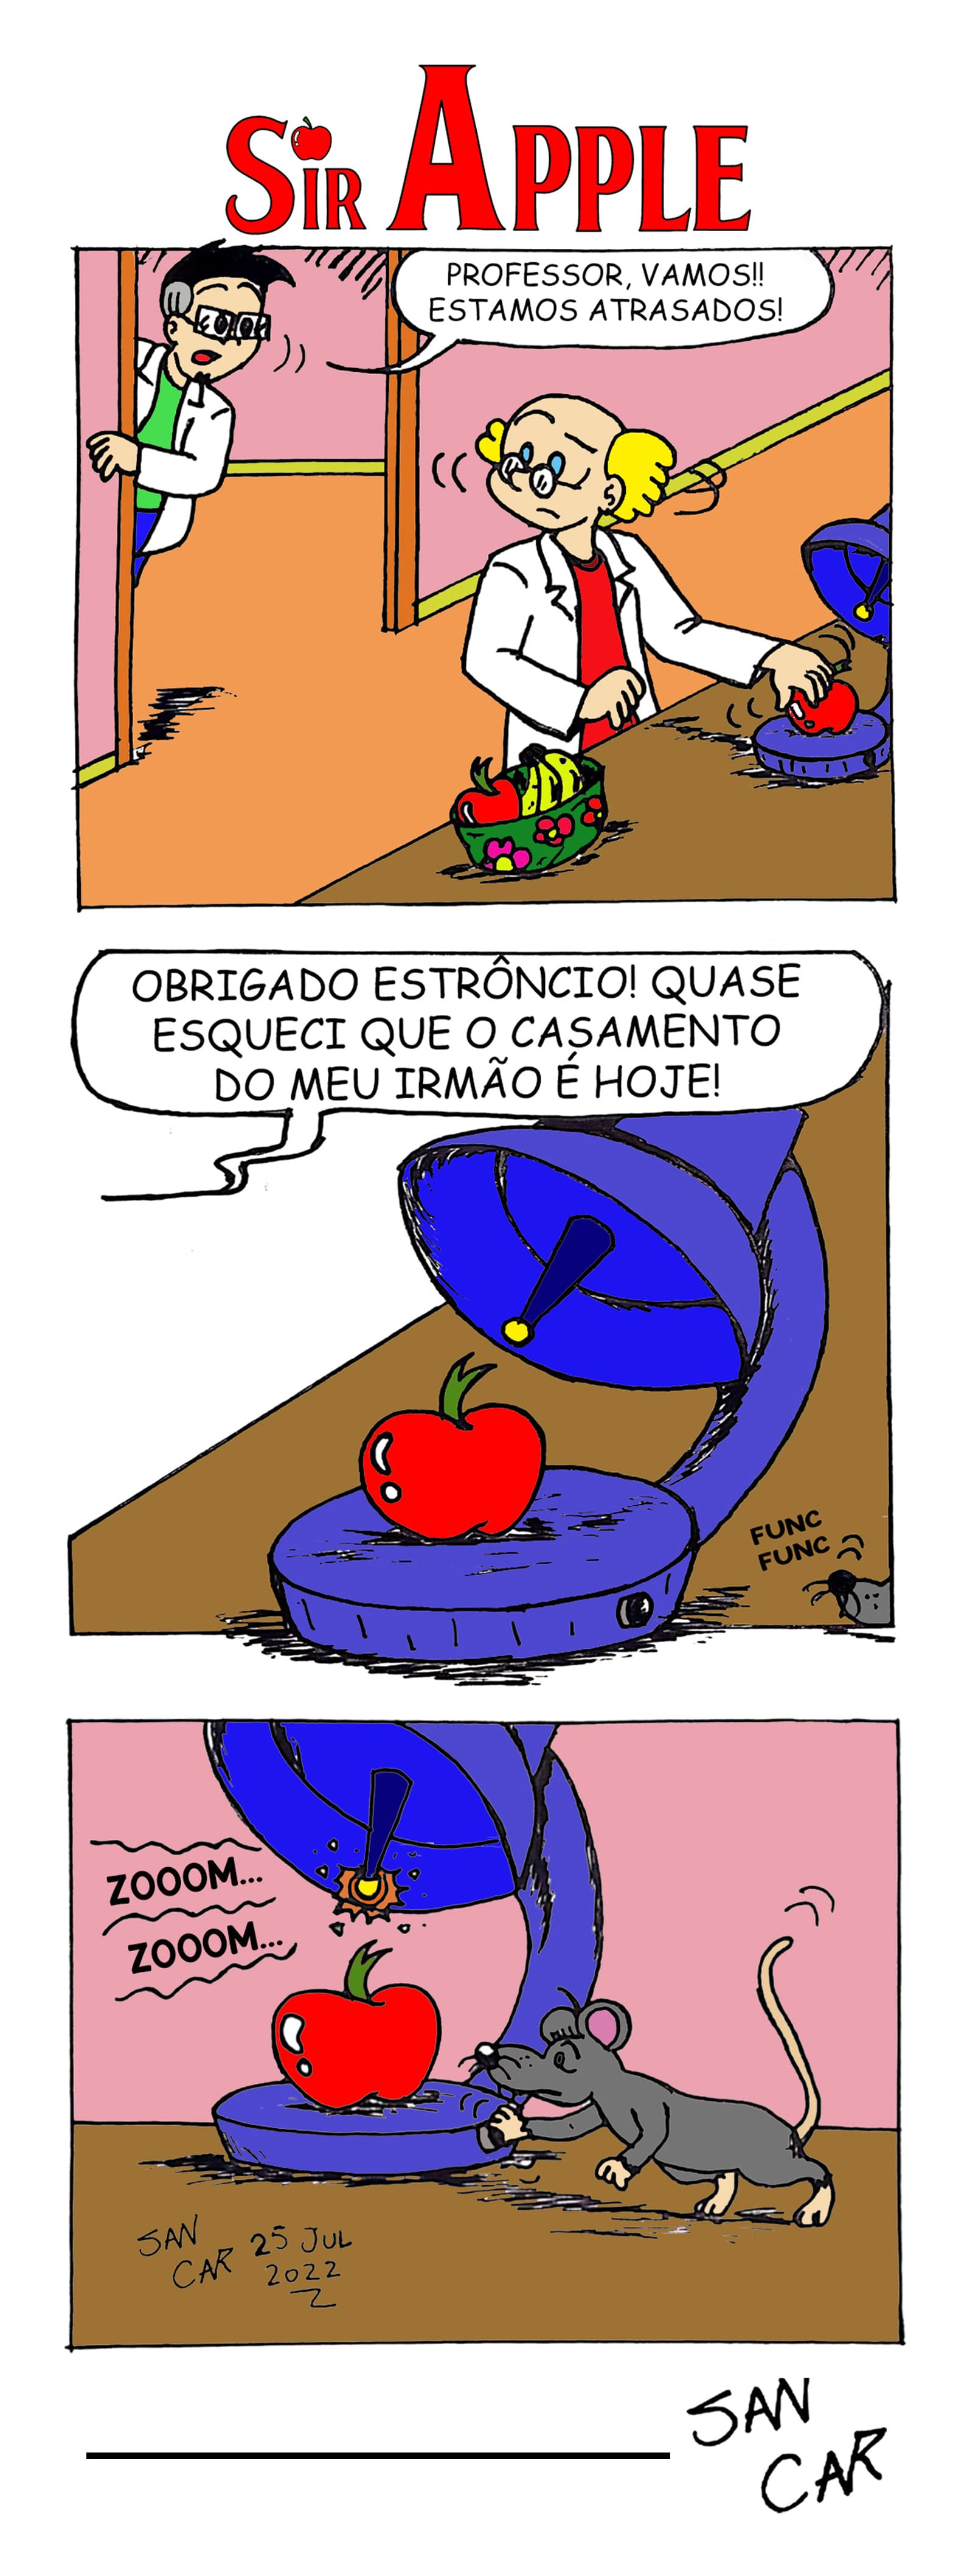
\includegraphics[width=\textwidth]{Tirinha/Tirinha_Fig/Tirinha_Sir_Apple.jpg}
\end{minipage}











    \newpage
\thispagestyle{empty}
% Linhas verticais Contra Capa
\begin{tikzpicture}[remember picture, overlay]
    \draw[line width=3.1cm, base] ($(current page.north east) - (0,0)$) -- ($(current page.south east) - (0,0)$);
    \draw[line width=1.05cm, base] ($(current page.north east) - (2.25,0)$) -- ($(current page.south east) - (2.25,0)$);
    \draw[line width=22.6cm, base] ($(current page.north east) - (14.25,0)$) -- ($(current page.south east) - (14.25,0)$);
\end{tikzpicture}

% Textos
\begin{tikzpicture}[remember picture, overlay]
  % Adiciona texto
  \node at (current page.north west) [anchor=north west, xshift=2cm, yshift=-3cm] {\begin{minipage}[t]{8cm} % Define a largura da minipage igual à largura da figura
  \setlength{\baselineskip}{1.5\baselineskip}
    {\sffamily\myfontsizeTemaCapaVerticalECC O Newston Jornal surgiu como uma iniciativa estudantil envolvendo alunos dos cursos de Física, Letras e Arquitetura e Urbanismo da Universidade Estadual de Maringá (UEM) em 2018, e foi oficializado como projeto de extensão vinculado oficialmente à universidade em março de 2021.} \end{minipage}
  };
   \node at (current page.north west) [anchor=north west, xshift=2cm, yshift=-10cm] {\begin{minipage}[t]{8cm} % Define a largura da minipage igual à largura da figura
  \setlength{\baselineskip}{1.5\baselineskip}
    {\sffamily\myfontsizeTemaCapaVerticalECC Desde o início, a finalidade do projeto consiste em produzir material para divulgação científica e cultural que atenda à comunidade externa e interna da universidade, visando sempre a integração de diversas áreas do conhecimento.} \end{minipage}
  };
\end{tikzpicture}

% Logo do Newston e da UEM
\begin{tikzpicture}[remember picture, overlay]
  % Adiciona a logo maçã branco
  \node at (current page.north west) [anchor=north west, xshift=1.8cm, yshift=-25.2cm] {
    
\includegraphics[width=6cm]{ContraCapa/Newston_Jornal_Logo_Horizontal_ContraCapa.png}
  };
  % Adiciona a logo da UEM Branco
  \node at (current page.north west) [anchor=north west, xshift=12.5cm, yshift=-25.7cm] {
    
\includegraphics[width=0.22\textwidth]{Capa/Figuras_Capa/UEM_Logo_Modelo_Branco.png}
  };
\end{tikzpicture}
    
\end{document}

% NOTAS

% Em certos momentos de compilação você pode obter "Package multicol Warning" para notas de rodapé ou figuras, verifique a disposição do seu texto no PDF e ignore esses erros caso não afetem o layout da edição nem a estética de acordo com a sua preferência. A mesma recomendação vale para mensagens de erros parecidas com "Underfull \hbox (badness 10000) in paragraph at lines X--X".

% CUIDADO COM IMAGENS GRANDES. Podem gerar conflitos com a versão gratuita do Overleaf devido a demora para compilar tais imagens com o documento.

% Comandos LaTeX desenvolvidos por Sanderson Carlos Ribeiro (e-mail: San.Car.Oficial@gmail.com) com o auxílio do ChatGPT. Design da Edição por Vítor Hugo Ribeiro (e-mail: vitorhibeiro@gmail.com) e Alexandre Alabora (e-mail: alexandre.alabora@gmail.com). Com contribuições de Luiz Felipe Demétrio (e-mail: demetrio.luizfelipe.fis@gmail.com).